\subsection{課題別の成否と費用}
表\ref{tab:p143-cells}と図\ref{fig:p143-cost}に全8条件を示す．
\begin{table*}[t]
\caption{課題別の成否と論理入出力．不明呼出しは0補完しない．差分付きactorは既知使用量の呼出し数．}
\ecaption{Task outcomes and logical input/output. Known subtotals are distinguished from unknown usage.}
\label{tab:p143-cells}
\centering
\begin{tabular}{llrrrl}
\hline
課題 & 方式 & 最終成否 & 既知token小計 & 不明呼出し & 差分付きactor \\ \hline
写真操作 & TR & 成功 & 200,016 & 0 & 0\\
写真操作 & TDO & 失敗 & 149,194 & 1 & 0\\
精算 & TR & 成功 & 182,483 & 0 & 0\\
精算 & TDO & 成功 & 218,061 & 0 & 13\\
返金 & TR & 成功 & 68,923 & 0 & 0\\
返金 & TDO & 成功 & 68,923 & 0 & 0\\
CSV処理 & TR & 失敗 & 194,187 & 0 & 0\\
CSV処理 & TDO & 失敗 & 110,147 & 0 & 6\\
\hline
\end{tabular}
\end{table*}
\begin{figure*}[t]
\centering
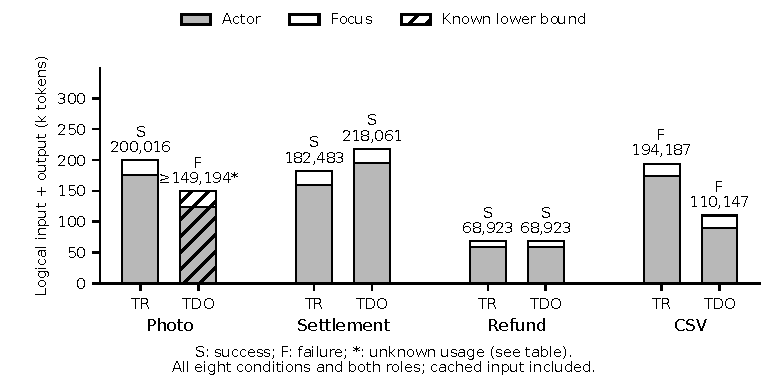
\includegraphics[width=130mm]{figures/p143_cost.pdf}
\caption{全8条件のactor・focus別論理入出力と最終成否．斜線は確定総費用ではない既知小計を示す．}
\ecaption{Logical input/output by role and final outcomes. Hatched bars denote known lower bounds.}
\label{fig:p143-cost}
\end{figure*}
\subsection{品質と全費用の比較}
全8条件を評価し，成功はTRが3/4，TDOが2/4だった．写真操作でTRの成功をTDOが失い，$L=1$となった．TDOの同課題はモデル呼出し中の時間上限で停止し，actor 1呼出しの使用量が不明だった．既知小計はTRが645,609，TDOが546,325トークンであるが，この差を総費用削減とは扱わない．固定した全8条件の会計充足条件を満たさないため，全体と共通成功集合の確定費用差・削減率はいずれも算出せず，効用条件と開発条件は不成立だった．

共通成功は精算と返金の2課題である．個別の確定値を見ると，精算はTDOが35,578トークン多く，返金は同値だった．CSV処理ではTDOが84,040トークン少なかったが，両方式ともAPI上限で停止し失敗した．この減少は，成功を保った節約の事例ではない．

\subsection{差分処置の作動範囲}
TDOの第2object focusは写真操作，精算，CSV処理の3課題で既知の送信を確認した．差分が採用されてactor入力に届いたのは精算とCSV処理の2/4課題で，差分付きの既知actor呼出しはそれぞれ13回，6回だった．返金では第2差分処置が作動しておらず，その成功を差分保持の効果例には数えない．写真操作でも差分付きactorは0回であり，旧要約保持が成功喪失の原因だとまでは特定できない．

差分が届いた唯一の共通成功課題である精算では，focus費用は52トークン減った一方，actor費用は35,630トークン増えた．旧要約の再出力を要求しない処置が，後続入力や行動を含む総費用の減少に直結しない実例である．ただし，増分を旧要約の保持量だけに帰属する比較ではなく，処置後の履歴と呼出し数の変化を含む．以上より，本条件では機構の作動は観測できたが，品質を保つ全仕事費用削減は確認できなかった．
